\begin{figure}[!htbp]
\centering
\vspace{1\baselineskip}
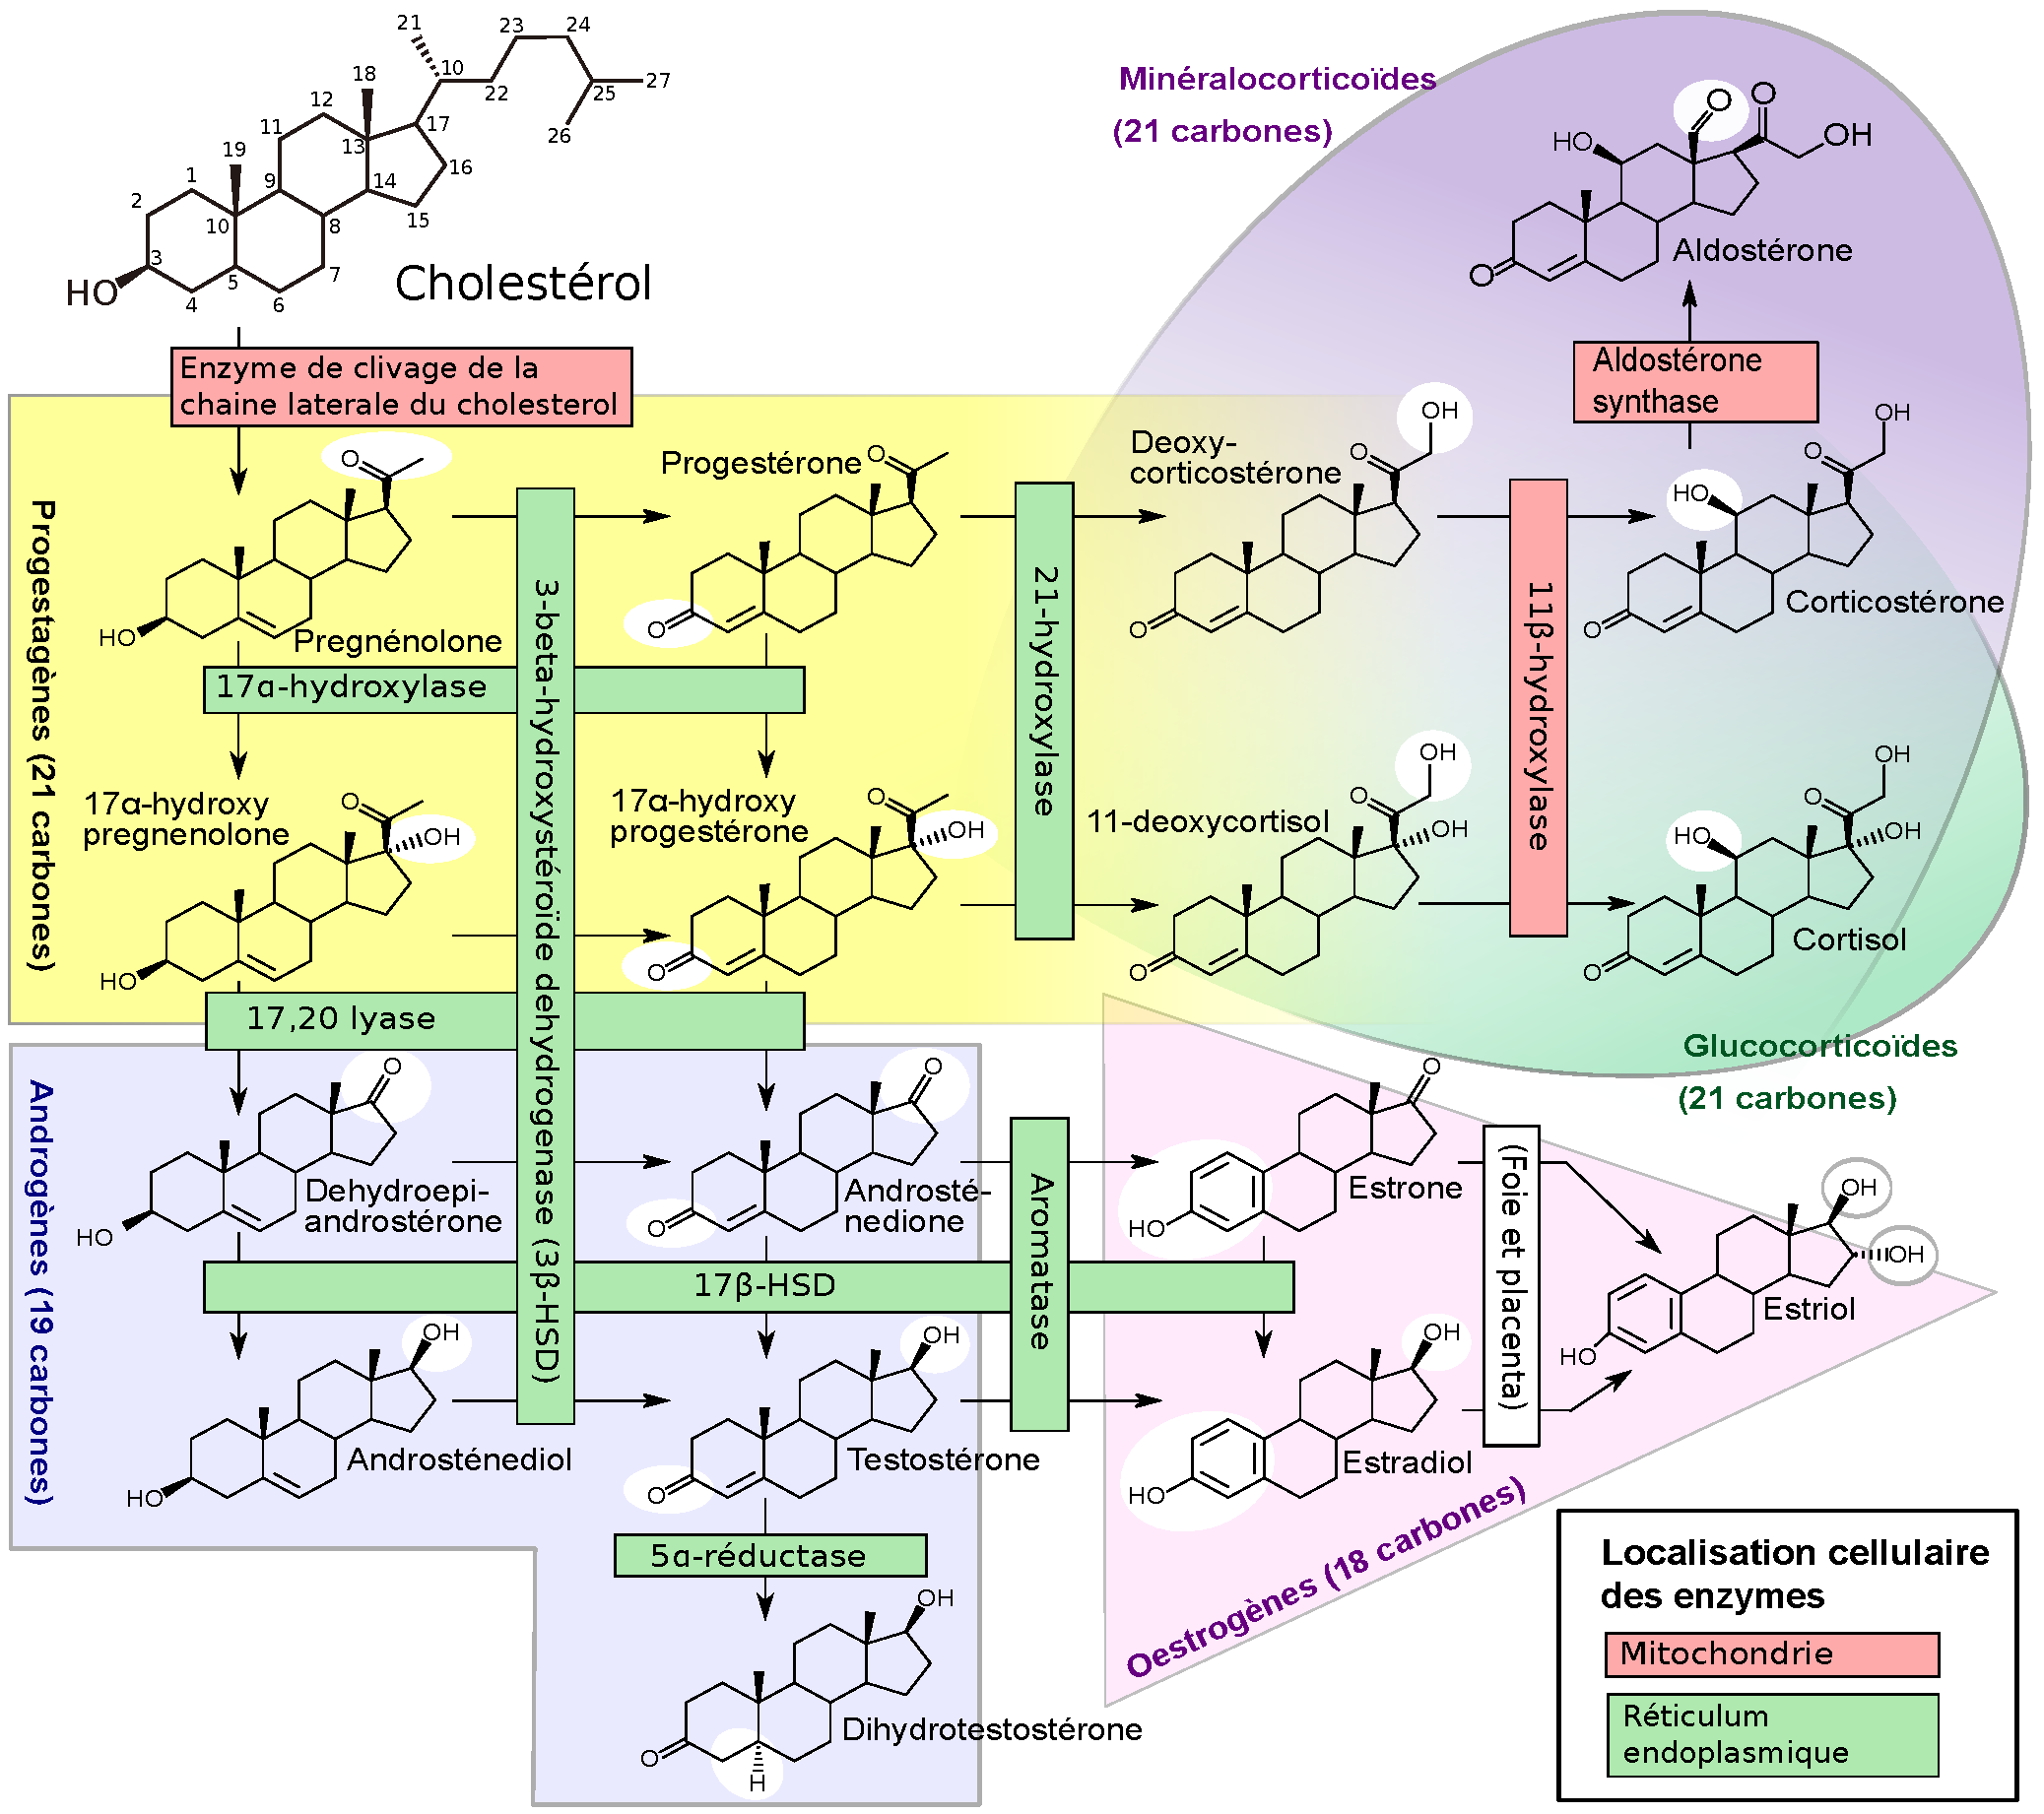
\includegraphics[width=\textwidth]
{Figures/steroidogenesis/steroidogenesis.pdf}
\caption[Principales étapes de la stéroidogenèse]
{
\glsreset{doc}\glsreset{cort}
Principales étapes de la stéroïdogenèse.
Le choléstérol est tout d'abord convertit en pregnénolone, qui à son tour est convertie en \gls{17aohpreg}, en \gls{17aohprog} ou en progestérone.
Ces deux dernières servent de précurseurs directs à l'obtention de 11-déoxycortisol et de \gls{doc}.
Enfin, par hydroxylation du 11-déoxycortisol et de la \gls{doc}, le cortisol et la \gls{cort} sont obtenus.
Les stéroïdes sexuels sont synthétisés à partir de \gls{17aohpreg} et de \gls{17aohprog} (partie inférieure du diagramme).
Tiré de "Steroidogenesis.svg" par David Richfield et Mikael Häggström.
}
\label{fig:steroidogenesis}
\end{figure}